\subsection{Разработка страницы заполнения медицинской карты}
В данной выпускной квалификационной работе разработка страницы заполнения медицинской карты является одним из важнейших аспектом приложения. Так как в медицинской карте присутствует очень много разнообразных полей для заполнений и со взглядом на будущее расширение, мной было принято создать удобный автоматический генератор этих полей. Моей основной задачей было создание такого генератора, благодаря которому можно было создать новый список вопросов в несколько простых действий.

Одной из важнейших частей процесса разработки такого генератора является использование шаблона проектирования \enquote{Компоновщик}. Это декомпозиционный шаблон, который представляет собой древовидную структуру классов и используется для представления иерархии часть-целое. В данном контексте, базовым классом в данной иерархии является TestQuestion. Этот класс определяет общий интерфейс для всех типов вопросов, а также содержит некоторые общие атрибуты и методы. Например, QuestionText используется для хранения текста вопроса, Options используется для хранения списка вариантов ответа, а методы GetValue и SetValue используются для получения и установки ответа на вопрос соответственно. Классы RadioButtonQuestion, CheckBoxQuestion и TextQuestion являются производными от класса TestQuestion и представляют различные типы вопросов. RadioButtonQuestion предназначен для вопросов с выбором одного ответа из списка, CheckBoxQuestion предназначен для вопросов с выбором нескольких ответов из списка, а TextQuestion предназначен для вопросов с текстовым ответом.

Классы RadioButtonWithTextQuestion и CheckBoxWithTextQuestion являются подклассами классов RadioButtonQuestion и CheckBoxQuestion соответственно. Они добавляют возможность ассоциировать дополнительный текст с вопросом с выбором. Это может быть полезно, когда необходимо добавить дополнительный текст к полю.

Структура классов представлена на рисунке~\ref{fig:questions}.

\begin{figure}
  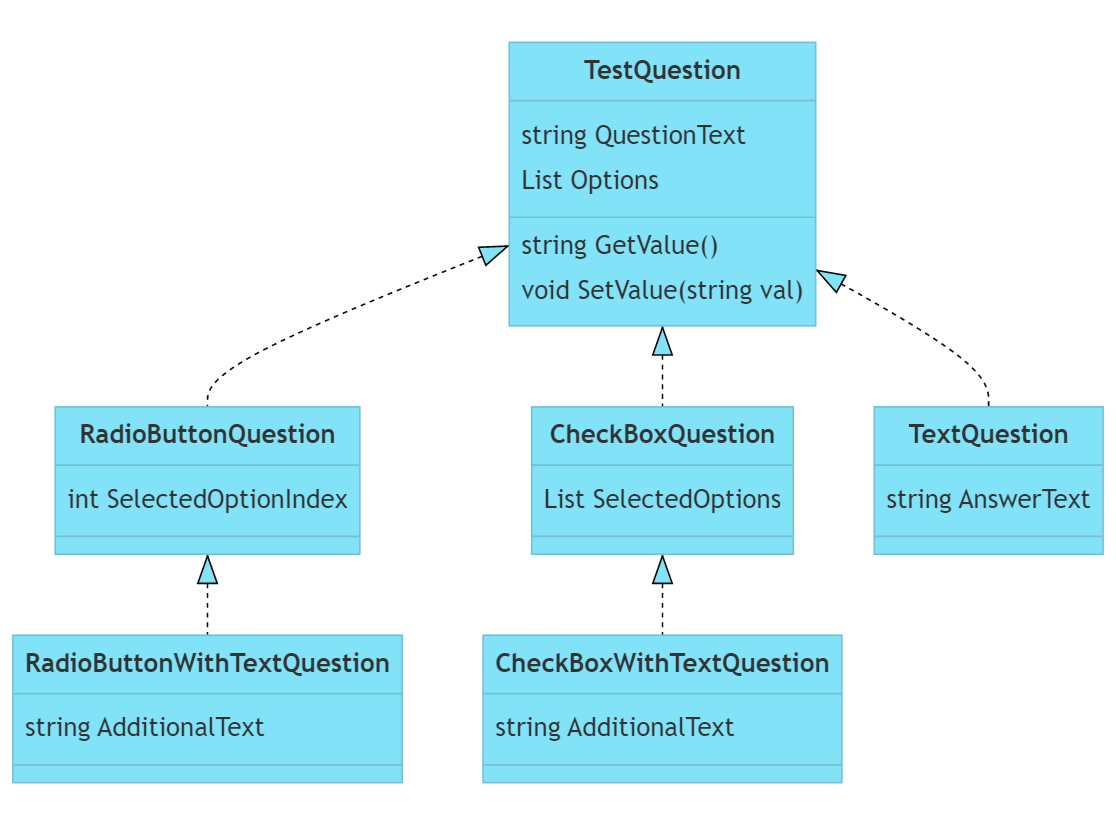
\includegraphics[scale=0.4]{inc/questions.png}
  \caption{Структура вопросов}
  \label{fig:questions}
\end{figure}


Для создания экземпляров классов вопросов используется класс TestQuestionsFactory. Это класс, который инкапсулирует логику создания объектов TestQuestion. Он использует информацию, содержащуюся в атрибутах свойств передаваемого объекта, для автоматической генерации вопросов и их настройки. В каждом цикле обработки свойств передаваемого объекта, TestQuestionsFactory проверяет наличие различных атрибутов, таких как RadioButtonQuestionAttribute, RadioButtonWithTextQuestionAttribute, CheckBoxQuestionAttribute, CheckBoxWithTextQuestionAttribute, TextQuestionAttribute. Если какой-то из этих атрибутов присутствует, создается соответствующий вопрос и добавляется в список testQuestions. Если у свойства есть значение, оно также устанавливается в созданном вопросе. Для каждого типа вопроса определен свой шаблон дизайна, то есть определена структура полей и внешний вид вопроса.

После того, как пользователь заполнил все поля, ответы сохраняются в экземпляре класса FullCard с помощью метода SaveTestResults. Этот метод итеративно обрабатывает все свойства FullCard, используя значения, возвращаемые методом GetValue каждого вопроса. Таким образом, результаты ответов пользователя переносятся в экземпляр класса FullCard. Пример кода класса FullCard на рисунке~\ref{src:question}.

\begin{figure}
\lstinputlisting[language=C++]{inc/questions.cs}
\caption{Класс FullCard}
\label{src:question}
\end{figure}

В результате такого подхода мы получаем гибко настраиваемый интерфейс страницы заполнения карты, который может отображать любой тип поля, определенный в нашей системе.